\documentclass[a4paper, 11pt, notitlepage,english]{article}

%
% Importering av pakker
%
\usepackage[utf8]{inputenc}
\usepackage[english]{babel}
\usepackage{lmodern}
\usepackage{algorithm,algorithmic}
\usepackage[T1]{fontenc, url}
\usepackage{textcomp}
\usepackage{amsmath, amssymb}
\usepackage{amsbsy, amsfonts}
\usepackage{graphicx, color}
\usepackage{listings}
\usepackage{multicol}
\usepackage{booktabs}
\usepackage{bbm}
\usepackage{amsthm}
\usepackage[text={6.2in,9.2in},centering]{geometry}
\usepackage{subfigure}
\bibliographystyle{plain}
 
\definecolor{dkgreen}{rgb}{0,0.6,0}
\definecolor{gray}{rgb}{0.9,0.9,0.9}
\definecolor{mauve}{rgb}{0.58,0,0.82}
 
\usepackage{parskip}
% \usepackage{tabularx}

%
% Parametere for inkludering av kode fra fil
%
%\lstset{language=python}
%\lstset{basicstyle=\ttfamily\small}
%\lstset{frame=single}
%\lstset{keywordstyle=\color{red}\bfseries}
%\lstset{commentstyle=\itshape\color{blue}}
%\lstset{showspaces=false}
%\lstset{showstringspaces=false}
%\lstset{showtabs=false}
%\lstset{breaklines}

\lstset{ %
    language=C++,
    backgroundcolor=\color{gray},
    basicstyle=\footnotesize,
    frame=bt,
    framexleftmargin=5pt,
    keywordstyle=\bf \color{dkgreen},
    commentstyle=\color{mauve}\slshape,
    breaklines=true
}

%
% Definering av egne kommandoer og miljøer
%
\newcommand{\dd}[1]{\ \text{d}#1}
\newcommand{\f}[2]{\frac{#1}{#2}} 
\newcommand{\beq}{\begin{equation*}}
\newcommand{\eeq}{\end{equation*}}
\newcommand{\bo}[1]{\boldsymbol{#1}}
\newcommand{\BAR}{%
  \hspace{-\arraycolsep}%
  \strut\vrule % the `\vrule` is as high and deep as a strut
  \hspace{-\arraycolsep}%
}
\newcommand{\norm}[1]{\left\lVert #1 \right\rVert}
\newcommand{\id}{\mathbbm{1}}
\newcommand{\idop}{\bbm 1}

\newtheorem{theorem}{Theorem}

%
% Navn og tittel
%
\author{Candidate numbers:}
\title{FYS4150 - Computational Physics \\
      Project 5: \\
       Diffusion of neurotransmitters in the synaptic cleft}

\begin{document}
\maketitle

\begin{abstract}
In this project we study diffusion of neurotransmitters in the brain across the synaptic cleft. In particular, we look at the solution to the diffusion equation for a particular choice of boundary conditions. Our choice of boundary conditions allows for an analytical solution that is found and later compared to the numerical results. The numerical solutions are found by use of three different integration schemes for partial differential equations: the Forward Euler scheme, the Backward Euler scheme and the Crank-Nicolson scheme. Finally, we compare these deterministic schemes to an implementation based on Monte Carlo methods and random walks. We find that ...\texttt{blah, results, blah}... \\
\end{abstract}

\begin{itemize}
\item Github repository link with all source files and benchmark calculations: \\
 \textcolor{blue}{https://github.com/henrisro/Project5}.
\item A list of all the code files can be found in the code listing in the end of this document.
\end{itemize}

\section{Introduction}

Diffusion of signal molecules is the dominant way of transportation in the brain. In this project we are going to study the solutions to the diffusion equation with restriction to some special boundary conditions. The basic process is illustrated in figure \ref{fig:Synaptic_cleft}. In (1) the vesicles inside the axon approach the presynaptic membrane and merge with it in (2). The vesicle contains neurotransmitters and release them across the synaptic cleft (of with $d$) in (3). If we denote the concentration of neurotransmitters at distance $x$ and time $t$ from the presynaptic membrane by $u(x,t)$, the dynamics can be described with the diffusion equation:

\begin{equation}
\frac{\partial u(x,t)}{\partial t} = D \nabla^2 u(x,t),
\label{eq:Diffusion_eq}
\end{equation}

where $\nabla^2 = \frac{\partial^2}{\partial x^2}$ in the one dimensional case. This equation will be the subject of investigations with restrictions to the interval $x\in [0,d]$ for $d=1$ and diffusion constant equal to unity $D=1$. We will apply the boundary conditions

\begin{equation}
u(0,t) = 1 \hspace{2mm} \forall t > 0 \hspace{10pt} \mathrm{and} \hspace{10pt} u(d,t) = 0 \hspace{2mm} \forall t > 0,
\label{eq:Boundary_condition}
\end{equation}

corresponding to a constant release of neurotransmitters at the presynaptic membrane ($u(0,t)$) and a constant absorption of transmitters at the postsynaptic membrane (at $u(d,t)$) at all times. The initial conditions will be taken to be:

\begin{equation}
u(x,t) = \begin{cases} 1  & \mathrm{if} \hspace{2mm} x = 0 \\
0  & \mathrm{if} \hspace{2mm} x \in(0,d] \end{cases} 
\label{eq:Initial_conditions}
\end{equation}

This basically means that all the neurotransmitters are located at $x=0$ initially when the vesicles are opened. \\

\begin{figure}[h!tb]
 \centering
 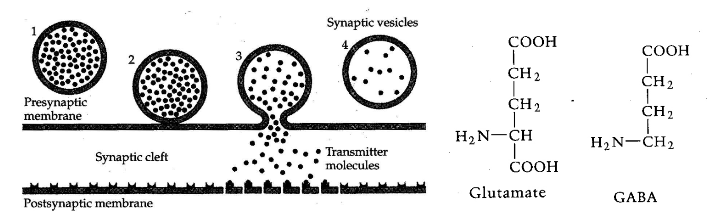
\includegraphics[width=0.9\textwidth]{Synaptic_cleft_project}
 \caption{Left: Illustration of the release of vesicle from an axon. The neurotransmitters (two chemical structures are shown to the right) travel diffusively across the synaptic cleft and are absorbed in the postsynaptic membrane at a distance $d$ away from the release point. The figure is taken from the project description \cite{Komp3150}, but originates from Thompson: "The Brain", Worth Publ., 2000.}
\label{fig:Synaptic_cleft}
\end{figure}

The solutions will be studied by implementation of three different deterministic schemes in addition to a Monte Carlo based method. We will look in some detail at the Forward Euler scheme, the Backward Euler scheme and the Crank-Nicholson scheme for partial differential equations (PDEs). The methods are compared in terms of precision and stability. 

\section{Theory}

In this section we derive the analytical solution to the diffusion problem outlined above. The closed form expression of the solution, although it will take the form of an infinite sum, will be valuable in terms of judging the numerical results later. 

\subsection{Analytical solution}
To solve the one dimensional diffusion equation, 

\begin{equation}
\frac{\partial u}{\partial t} = \frac{\partial^2 u}{\partial x^2},
\label{eq:Basic_problem}
\end{equation}

with the boundary conditions in (\ref{eq:Boundary_condition}) and initial conditions in (\ref{eq:Initial_conditions}), we apply the standard \emph{separation of variables} ansatz:

\begin{equation}
 u(x,t) = X(x)T(t) + u_s(x)
\label{eq:Separation of variables}
\end{equation}

We here separate out the steady-state solution $u_s(x) = 1-x$, which trivially satisfies equation (\ref{eq:Basic_problem}). When inserted into equation (\ref{eq:Basic_problem}) we arrive at:

\begin{equation}
\frac{1}{X} \frac{d^2 X}{dx} = \frac{1}{T}\frac{dT}{dt} = -k^2
\label{eq:Separated_equation}
\end{equation}

The last equality (i.e. both sides equal to a constant) follows since the left hand side is independent of $t$ and the right hand side independent of $x$. Looking first at the $X(x)$ equation, we realize that it is simply the harmonic oscillator equation with solution $X(x) = a\cos(kx) + b\sin(kx)$. The boundary condition in equation (\ref{eq:Boundary_condition}) translates to (since we must have $X(0) = X(1) = 0$ after adding the steady-state solution) $a = 0$ and $\sin(k) = 0 \Rightarrow k_n = n\pi$ for $n \in \mathbb{N}$. We thus have:

\begin{equation}
X_n(x) = b_n \sin(n\pi)
\label{eq:Separated_X_solution}
\end{equation}

The equation for $T(t)$ is a separable first order differential equation and have solutions:

\begin{equation}
T_n(x) = \exp(-(n\pi)^2t)
\label{eq:Separated_T_solution}
\end{equation}

The general solution is then a sum of (possibly all) the modes $X_n(x)T_n(t)$:

\begin{equation}
u(x,t) = 1-x +\sum_{n=1}^{\infty} b_n \sin(n\pi x) e^{-(n\pi)^2t}
\label{eq:General_solution}
\end{equation}

The final step is to determine the coefficients $b_n$ such that $u(x,0)$ fits the initial conditions in equation (\ref{eq:Initial_conditions}). This can be rewritten as 

\begin{equation}
\sum_{n=1}^{\infty} b_n \sin(n\pi x) = u_0(x) =  \begin{cases} 0 & \mathrm{if} \hspace{2mm} x = 0 \\
x-1 & \mathrm{if} \hspace{2mm} x \in (0,1] \end{cases}
\label{eq:Initial_cond_fit}
\end{equation}

This is just as the Fourier series of the odd extension of the function $u_0(x)$ on the interval $[0,1]$. The coefficients are determined by Fourier's trick (see for instance \cite{Boas}):

\begin{equation}
b_n = 2\int_0^1 dx \hspace{1mm} (x-1) \sin(n\pi x) = -\frac{2}{n\pi}
\label{eq:Fourier_trick}
\end{equation}

We hence have arrived at the final closed form solution:

\begin{equation}
\boxed{u(x,t) = 1-x - \frac{2}{\pi} \sum_{n=1}^{\infty} \frac{\sin(n\pi x)}{n} e^{-(n\pi)^2t}}
\label{eq:Final_solution}
\end{equation}

\subsection{Stability of matrix iterations}
Suppose we are given the iteration $\boldsymbol{V}_i = A \boldsymbol{V}_{i-1}$ for some matrix $A$ and vectors $\boldsymbol{V}_i$. This implies that the vector after $n$ iterations is given in terms of the initial one as: $\boldsymbol{V}_n = A^n \boldsymbol{V}_0$. By expanding $\boldsymbol{V}_0$ in the eigenvector basis of $A$, we can quickly understand the following theorem quite intuitively: \\

\begin{theorem}
The solution to the iteration $\boldsymbol{V}_i = A \boldsymbol{V}_{i-1}$ will converge to a definite value if $\rho(A) < 1$, where $\rho(A)$ is the spectral radius of $A$:

\begin{equation}
\rho(A) = \mathrm{max}\{\lvert \lambda_n \rvert : \mathrm{det}(A-\lambda_n\id)=0 \}
\label{eq:Spectral_radius}
\end{equation}
\end{theorem}

This is a central concept in Chaos theory when determining for example the stability of flows and maps\footnote{This is for instance covered in Predrag Cvitanović's book on chaos theory: http://chaosbook.org/.}.

\section{Method / Algorithm}
This section is devoted to the discussion of the three deterministic schemes for PDEs mentioned earlier. We derive the algorithms and investigate their stability properties expressed in terms of $\Delta x$ and $\Delta t$. First some general nomenclature. We discretize the interval $[0,1]$ with a step length determined by some integer $n$: 

\begin{equation}
 \Delta x = \frac{1}{n+1}
\label{eq:Step_length}
\end{equation}

such that $x \mapsto x_i = i\Delta x$ for $i \in \{0,1,\dots,n+1 \}$. A corresponding discretization in time is given by $\Delta t$ (we will later discuss how this should be chosen depending on $\Delta x$, i.e. $n$). This means that $t\mapsto t_j = j\Delta t$ for $j\in \mathbb{N}$. The following discussion will be made in the context of the diffusion equation, here written compactly as $u_{xx} = u_t$ (the subscripts refer to derivatives). After discretization we use the notation $u(x,t) \mapsto u(x_i, t_j) \equiv u_{i,j}$. The following definition will also appear frequently in what follows:

\begin{equation}
 \alpha \equiv \frac{\Delta t}{\Delta x^2}
\label{eq:Step_parameter}
\end{equation}

The following discussion and derivations follow \cite{Komp3150} closely.

\subsection{Forward Euler scheme}
In this scheme we use the two simplest possible approximations for the derivatives $u_{xx}$ and $u_t$:

\begin{equation}
u_{xx} \approx \frac{u(x+\Delta x,t)-2u(x,t)+u(x-\Delta x, t)}{\Delta x^2} \mapsto \frac{1}{\Delta x^2} (u_{i+1,j}-2u_{i,j}+u_{i-1,j})
\label{eq:Forward_uxx}
\end{equation}

and

\begin{equation}
u_{t} \approx \frac{u(x,t+\Delta t)-u(x, t)}{\Delta t} \mapsto \frac{1}{\Delta t} (u_{i,j+1}-u_{i,j})
\label{eq:Forward_ut}
\end{equation}

This leads directly to an explicit scheme when equating the above expressions:

\begin{align}
u_{xx} &= u_t \Rightarrow \\
 \frac{1}{\Delta x^2} (u_{i+1,j}-2u_{i,j}+u_{i-1,j}) &= \frac{1}{\Delta t} (u_{i,j+1}-u_{i,j}) \Rightarrow \\
 u_{i,j+1} &= \alpha u_{i+1,j} + (1-2\alpha)u_{i,j} + \alpha u_{i-1,j}
\label{eq:Forward_Euler_scheme}
\end{align}

\begin{figure}[h!tb]
 \centering
 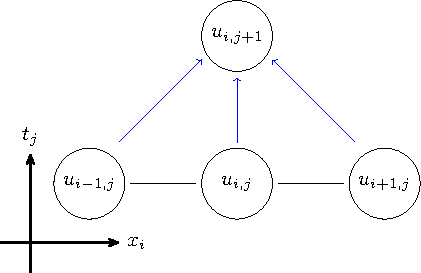
\includegraphics[width=0.4\textwidth]{Grid_FE-figure0}
 \caption{Forward Euler computational grid scheme for the $(1+1)$-dimensional diffusion equation. $u_{i,j}$ is the discretized solution at position $x_i$ and time $t_j$.}
 \label{fig:FE_grid}
\end{figure}

This scheme is explicit in the sense that it gives a recipe of how to find the solution at the next time step given the solution at the previous one. It should be initialized with the initial condition, $u_{i,0} = u_0(x_i)$ as given in equation (\ref{eq:Initial_cond_fit}). In terms of a matrix equation we can write:

\begin{align}
\boldsymbol{U}_{j+1} &= A \boldsymbol{U}_j \\
\begin{bmatrix}
u_{1,j+1} \\ u_{2,j+1} \\ \vdots \\ u_{n,j+1}
\end{bmatrix}
&=
\begin{bmatrix}
 1-2\alpha & \alpha & 0 & \cdots & 0 & 0 \\
 \alpha & 1-2\alpha & \alpha & \cdots & 0 & 0 \\
  & \vdots & & \ddots & & \vdots \\
 0 & 0 & 0 & \cdots & \alpha & 1-2\alpha \\
\end{bmatrix}
\begin{bmatrix}
u_{1,j} \\ u_{2,j} \\ \vdots \\ u_{n,j}
\end{bmatrix}
\label{eq:Forward_Euler_matrix}
\end{align}

with the initial condition (in our case) $\boldsymbol{U}_0 = ( u_0(\Delta x), u_0(2\Delta x), \dots, u_0(1))^T = (1,0,\dots,0)^T$. It is appropriate, also for later reference, to decompose the matrix as $A = \id - \alpha B$ where the elements of $B$ can be expressed in terms of Kronecker deltas: 

\begin{equation}
B_{i,j} = 2\delta_{i,j}-\delta_{i+1,j}-\delta_{i-1,j}
\label{eq:Matrix_B}
\end{equation}

The subscripts here refer to matrix indices and have nothing to do with time and space coordinates as earlier. \\

\textbf{Truncation errors} \newline
The discretized equations in (\ref{eq:Forward_uxx}) and (\ref{eq:Forward_ut}) are easily seen to come from the Taylor expansions (with step lengths $\Delta x$ and $\Delta t$ respectively) around $u(x,t)$ 

\begin{align}
u(x\pm\Delta x,t) &= u(x,t) \pm \frac{\partial u(x,t)}{\partial x}\Delta x + \frac{\partial^2 u(x,t)}{\partial x^2}\Delta x^2 + \mathcal{O}(\Delta x^3)
\label{eq:Forward_Euler_expansions1} \\
u(x,t\pm \Delta t) &= u(x,t) \pm \frac{\partial u(x,t)}{\partial t}\Delta t + \mathcal{O}(\Delta t^2)
\label{eq:Forward_Euler_expansions2}
\end{align}

and spell out for us that the Forward Euler scheme gives rise to errors of orders $\mathcal{O}(\Delta t)$ and $\mathcal{O}(\Delta x^2)$ when inserted into (\ref{eq:Forward_uxx}) and (\ref{eq:Forward_ut}). \\

\textbf{Stability condition} \newline
To determine for what combinations of $\Delta t$ and $\Delta x$ the Forward Euler scheme is stable, we investigate the spectral radius of the matrix $B$ (the other part of $A = \id - \alpha B$ is proportional to $\id$ and gives rise to a simple unit contribution to the eigenvalues):

\begin{align}
(B\boldsymbol{v})_i &= \lambda_i v_i \\
\sum_{j=1}^n [2\delta_{i,j}-\delta_{i+1,j}-\delta_{i-1,j}]v_j &= \lambda_i v_i
\label{eq:Forward_Euler_stability1}
\end{align}

We continue with expanding the vector components in a sine basis $v_i = \sin(i\theta)$ with $\theta = $ such that

\begin{align}
\sum_{j=1}^n [2\delta_{i,j}-\delta_{i+1,j}-\delta_{i-1,j}]v_j &= \lambda_i v_i \\
2 \sin(i\theta) - \sin\left((i+1)\theta\right) - \sin\left((i-1)\theta\right) &= \lambda_i \sin(i\theta) \\
2(1-\cos(\theta)) &= \lambda_i
\label{eq:Forward_Euler_stability2}
\end{align}

Hence in order to have $\rho(A) < 1$, we must have

\begin{equation}
\lvert 1-2\alpha(1-\cos(\theta)) \rvert < 1 \Rightarrow \alpha = \frac{\Delta t}{\Delta x^2} \leq \frac{1}{2}
\label{eq:Forward_Euler_stability3}
\end{equation}

The extremal eigenvalue occurs when $\theta = \pi$, at which the final inequality follows.

\subsection{Backward Euler scheme}
The Backward Euler scheme (just like for ordinary differential equations) exploits a time derivative approximation with a function evaluation backwards in time and the same approximation for $u_{xx}$ as in equation (\ref{eq:Forward_uxx}). We (re)state both approximations to have a clear argument:

\begin{equation}
u_{xx} \approx \frac{u(x+\Delta x,t)-2u(x,t)+u(x-\Delta x, t)}{\Delta x^2} \mapsto \frac{1}{\Delta x^2} (u_{i+1,j}-2u_{i,j}+u_{i-1,j})
\label{eq:Backward_uxx}
\end{equation}

and

\begin{equation}
u_{t} \approx \frac{u(x,t)-u(x,t-\Delta t)}{\Delta t} \mapsto \frac{1}{\Delta t} (u_{i,j}-u_{i,j-1})
\label{eq:Backward_ut}
\end{equation}

Equating these leaves us with:

\begin{align}
u_{xx} &= u_t \Rightarrow \\
 \frac{1}{\Delta x^2} (u_{i+1,j}-2u_{i,j}+u_{i-1,j}) &= \frac{1}{\Delta t} (u_{i,j}-u_{i,j-1}) \Rightarrow \\
 u_{i,j-1} &= -\alpha u_{i+1,j} + (1+2\alpha)u_{i,j} - \alpha u_{i-1,j}
\label{eq:Backward_Euler_scheme}
\end{align}

\begin{figure}[h!tb]
 \centering
 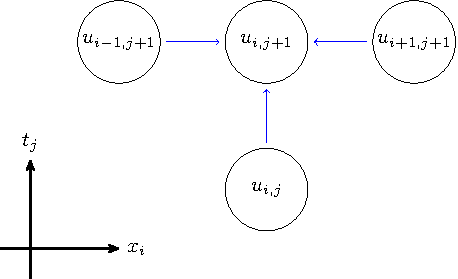
\includegraphics[width=0.4\textwidth]{Grid_BE-figure0}
 \caption{Backward Euler computational grid scheme for the $(1+1)$-dimensional diffusion equation. $u_{i,j}$ is the discretized solution at position $x_i$ and time $t_j$.}
 \label{fig:BE_grid}
\end{figure}

This recursion relation backwards in time does, as compared to the Forward Euler scheme, not give us the solution for the next time step in terms of the previous one. It instead takes the following form when written in matrix notation:

\begin{align}
C \boldsymbol{U}_j &= \boldsymbol{U}_{j-1} \\
\begin{bmatrix}
 1+2\alpha & -\alpha & 0 & \cdots & 0 & 0 \\
 -\alpha & 1+2\alpha & -\alpha & \cdots & 0 & 0 \\
  & \vdots & & \ddots & & \vdots \\
 0 & 0 & 0 & \cdots & -\alpha & 1+2\alpha \\
\end{bmatrix}
\begin{bmatrix}
u_{1,j} \\ u_{2,j} \\ \vdots \\ u_{n,j}
\end{bmatrix}
&=
\begin{bmatrix}
u_{1,j-1} \\ u_{2,j-1} \\ \vdots \\ u_{n,j-1}
\end{bmatrix}
\label{eq:Backwards_Euler_matrix}
\end{align}

with $C = \id + \alpha B$ and $B$ is the same as in (\ref{eq:Matrix_B}). This asks for, at each time step $j$, nothing else than a set of linear equations to be solved. Phrased differently, a matrix inversion (meaning we must find $C^{-1}$ with $C$ tridiagonal as above) would give us the solution at each time step straight away: $\boldsymbol{U}_j = C^{-1} \boldsymbol{U}_{j-1}$. However, a matrix-vector multiplication at each time step is computationally consuming as it costs $\mathcal{O}(n^2)$ FLOPS and the matrix inversion even worse with its $\mathcal{O}(n^3)$ FLOPS. From Project 1, however, we know that solving such equations for a tridiagonal matrix can be done by an algorithm that takes only $\mathcal{O}(n)$ FLOPS; far superior when the dimension becomes large. \\

\textbf{Truncation errors} \newline
Equations in (\ref{eq:Backward_uxx}) and (\ref{eq:Backward_ut}), just as for the Forward Euler scheme, stem from the Taylor expansions (with step lengths $\Delta x$ and $\Delta t$ respectively) as in equation (\ref{eq:Forward_Euler_expansions1}) and (\ref{eq:Forward_Euler_expansions2}). It is straight forwardly seen that this scheme gives identical truncation errors – of orders $\mathcal{O}(\Delta t)$ and $\mathcal{O}(\Delta x^2)$ – just as in the explicit method. \\

\textbf{Stability condition} \newline
This time we need to consider the spectral radius of $C^{-1} = (\id + \alpha B)^{-1}$. However, the work done in the stability discussion of the Forward Euler method gives us the answer quickly. We know from the earlier discussion that the eigenvalues of $C$ are strictly positive and larger than unity: $\mu_i = 1 + 2\alpha(1-\cos(\theta)) > 1$. This implies that the eigenvalues of $C^{-1}$ are strictly less than $1$: $\mu_i^{-1} < 1$. Furthermore we have $\rho(C^{-1}) < 1$ for all combinations of $\Delta t$ and $\Delta x$; a rather weak stability condition (i.e. no restrictions on the step lengths).

\subsection{Crank-Nicolson scheme}
The Crank-Nicolson scheme is, in a sense, an equally weighted compromise between the forward Euler scheme and the backward Euler scheme. To see this explicitly, let us rephrase and compare the two previous schemes:

\begin{equation}
 \frac{1}{\Delta t} (u_{i,j}-u_{i,j-1}) = \frac{1}{\Delta x^2} (u_{i+1,j-1}-2u_{i,j-1}+u_{i-1,j-1}) \hspace{10pt} \mathrm{(Forward \hspace{2mm} Euler)}
\end{equation}

\begin{equation}
 \frac{1}{\Delta t} (u_{i,j}-u_{i,j-1}) = \frac{1}{\Delta x^2} (u_{i+1,j}-2u_{i,j}+u_{i-1,j}) \hspace{10pt} \mathrm{(Backward \hspace{2mm} Euler)}
\end{equation}

Adding the two equations gives the Crank-Nicolson scheme\footnote{A more general approach would be to assign different weights the two contributions in what is known as a $\theta$-rule \cite{Komp3150}.}:

\begin{align}
\frac{2}{\Delta t} (u_{i,j}-u_{i,j-1}) &= \frac{1}{\Delta x^2} (u_{i+1,j}-2u_{i,j}+u_{i-1,j}+u_{i+1,j}-2u_{i,j}+u_{i-1,j} ) \Rightarrow \\
 -\alpha u_{i+1,j} + 2(1+\alpha)u_{i,j} -\alpha u_{i-1,j} &= \alpha u_{i+1,j-1} + 2(1-\alpha) u_{i,j-1} + \alpha u_{i-1,j-1}
\label{eq:Crank_Nicoloson_scheme}
\end{align}

\begin{figure}[h!tb]
 \centering
 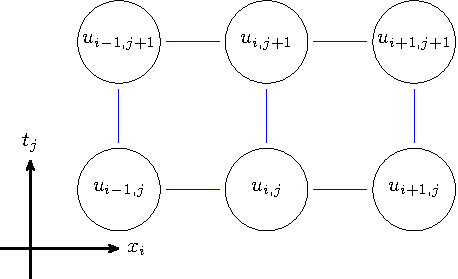
\includegraphics[width=0.4\textwidth]{Grid_CN-figure0}
 \caption{Crank-Nicolson computational grid scheme for the $(1+1)$-dimensional diffusion equation. $u_{i,j}$ is the discretized solution at position $x_i$ and time $t_j$.}
 \label{fig:CN_grid}
\end{figure}


or in matrix notation:

\begin{align}
(2\id + \alpha B) \boldsymbol{U}_j &= (2\id - \alpha B) \boldsymbol{U}_{j-1} \\
\begin{bmatrix}
 2+2\alpha & -\alpha & 0 & \cdots & 0 & 0 \\
 -\alpha & 2+2\alpha & -\alpha & \cdots & 0 & 0 \\
  & \vdots & & \ddots & & \vdots \\
 0 & 0 & 0 & \cdots & -\alpha & 2+2\alpha \\
\end{bmatrix}
\begin{bmatrix}
u_{1,j} \\ u_{2,j} \\ \vdots \\ u_{n,j}
\end{bmatrix}
&= \\
\begin{bmatrix}
 2-2\alpha & \alpha & 0 & \cdots & 0 & 0 \\
 \alpha & 2-2\alpha & \alpha & \cdots & 0 & 0 \\
  & \vdots & & \ddots & & \vdots \\
 0 & 0 & 0 & \cdots & \alpha & 2-2\alpha \\
\end{bmatrix}
&\begin{bmatrix}
u_{1,j-1} \\ u_{2,j-1} \\ \vdots \\ u_{n,j-1}
\end{bmatrix}
\label{eq:Crank_Nicolson_matrix}
\end{align}

Thus $\boldsymbol{U}_j = (2\id+\alpha B)^{-1}(2\id - \alpha B)\boldsymbol{U}_{j-1}$. This looks very similar to the Backward Euler scheme with the only difference that we must at each time step first calculate $\tilde{\boldsymbol{U}}_{j-1} = (2\id - \alpha B)\boldsymbol{U}_{j-1}$ before sending $(2\id + \alpha B)\boldsymbol{U}_j = \tilde{\boldsymbol{U}}_{j-1}$ to the tridiagonal matrix solver. \\

\textbf{Truncation errors} \newline
The Crank-Nicolson scheme was presented above as the sum of two equally weighted contributions to $u_t$ – at steps $j+1$ and $j$ (figure \ref{fig:CN_grid}). The formulas for $u_{xx}$ were not altered, so the truncation errors in $x$ are still of the same order $\mathcal{O}(\Delta x^2)$. To see what happens to the truncation in $t$, we can Taylor expand the involved quantities around $t' = t + \Delta t /2$ and only care about the errors in powers of $\Delta t$:

\begin{align}
u(x\pm\Delta x,t) &= u(x,t') \pm \frac{\partial u(x,t')}{\partial x}\Delta x + \frac{\partial^2 u(x,t')}{\partial x^2}\Delta x^2 + \\
&+ \frac{\partial u(x,t')}{\partial t}\frac{\Delta t}{2} + \frac{\partial^2 u(x,t')}{\partial t^2}\frac{\Delta t^2}{4} \pm \frac{\partial^2 u(x,t')}{\partial x \partial t}\frac{\Delta x \Delta t}{2} + \mathcal{O}(\Delta t^3)
\label{eq:Crank_Nicolson_expansions1} \\
u(x\pm\Delta x,t) &= u(x,t') \pm \frac{\partial u(x,t')}{\partial x}\Delta x + \frac{\partial^2 u(x,t')}{\partial x^2}\Delta x^2 + \\
&- \frac{\partial u(x,t')}{\partial t}\frac{\Delta t}{2} + \frac{\partial^2 u(x,t')}{\partial t^2}\frac{\Delta t^2}{4} \mp \frac{\partial^2 u(x,t')}{\partial x \partial t}\frac{\Delta x \Delta t}{2} + \mathcal{O}(\Delta t^3)
\label{eq:Crank_Nicolson_expansion2} \\
u(x,t+\Delta t) &= u(x,t') + \frac{\partial u(x,t')}{\partial t}\frac{\Delta t}{2} + \frac{\partial^2 u(x,t')}{\partial t^2}\frac{\Delta t^2}{4}  + \mathcal{O}(\Delta t^3)
\label{eq:Crank_Nicolson_expansion3} \\
u(x,t) &= u(x,t') - \frac{\partial u(x,t')}{\partial t}\frac{\Delta t}{2} + \frac{\partial^2 u(x,t')}{\partial t^2}\frac{\Delta t^2}{4}  + \mathcal{O}(\Delta t^3)
\label{eq:Crank_Nicolson_expansion4}
\end{align}

Putting these expansions carefully into equation (\ref{eq:Crank_Nicoloson_scheme}) (with the discretized labellings such as $u(x+\Delta x,t) = u_{i+1,j}$ etc.) and collecting the surviving terms, one does in fact see that the leading order truncation error in time is $\mathcal{O}(\Delta t^2)$ – an improvement as compared to the Forward and Backward Euler schemes. \\

\textbf{Stability condition} \newline
We need to look at the spectral radius of $(2\id + \alpha B)^{-1}(2\id -\alpha B)$. We can also this time reuse some earlier derived results. Recall the eigenvalues of $B$: $\lambda_i = 2(1-\cos(\theta) ) \in (0,4]$. The spectral radius condition thus translates to the following in this case:

\begin{equation}
\rho\left( (2\id + \alpha B)^{-1}(2\id -\alpha B) \right) = \frac{\lvert 2-\alpha \lambda_i\rvert}{\lvert 2+\alpha \lambda_i \rvert} < 1
\label{eq:Crank_Nicolson_spectralrad}
\end{equation}

This inequality is quite trivially seen to be satisfied since $\lambda_i > 0$. It is even more clearly seen by considering the two cases $\alpha\lambda_i < 2$ and $\alpha\lambda_i > 2$ separately. In total, we arrive at the same condition as for the Backward Euler scheme: all combinations of $\Delta t$ and $\Delta x$ results in a stable solution.

\subsection{Monte Carlo methods and random walks}

\section{Results}

\section{Discussion}
%\label{sec:Discuss}

\section{Conclusion}

\section{Appendix}

\bibliography{References_pro5}

\section*{Code listing}


 %\begin{equation}
 %\delta a = \delta \gamma\cos{\gamma}
%\label{eq:aksel_1_usikker}
%\end{equation}
 
 %\begin{table}[h!tb]
%\begin{center}
   %\begin{tabular}{ | p{2cm} | p{2cm} | p{3cm} |}
    %\hline
     %& $x_i$ [mm] & $\delta x_i$ [mm] \vspace{2 mm} \\ \hline
     %$l_a$ & 708 & 0   \\ 
     %$dl_s$ & 0 & 0.5  \\ 
     %$\sqrt{n}\cdot dl_l$ & 0 & $\sqrt{3}\cdot0.5 =0.87$  \\ 
     %$dl_m$ & 0 & $0.1\cdot\frac{708}{100} = 0.71$ \vspace{2 mm} \\ \hline
     %&$\sum_i x_i$ & $\sqrt{\sum_i \delta x_i}$  \\ 
     %& 708 & 1.12 \\ \hline
    %\end{tabular}
%\end{center}
%\caption{Måling av $x$ med målestokk. Til gjeldende antall siffer: $x = (708 \pm 1)$ mm.}
%\end{table}
 
 %\begin{figure}[h!tb]
 %\centering
 %\mbox{\subfigure{\includegraphics[width=2.7in]{kjent_vinkel_skraaplan}}\quad
 %\subfigure{\includegraphics[width=2.7in]{kjent_vinkel_skraaplan_linreg} }}
 %\caption{Til venstre: Hastighet som funksjon av tid mens bilen trillet langs skråplanet. Til høyre: Lineær regresjon på partiet der hastigheten øker jevnt.}
%\end{figure}

%\begin{figure}[h!tb]
 %\centering
 %includegraphics[width=2.7in]{Raynold_Rayleigh}
 %\caption{Plott av data fra tabell 2, dvs. Raynoldstallet plottet mot henholdsvis Rayleigh- og Stokes-koeffisientene for de ulike kombinasjonene av ballonger og vekter.}
%\end{figure}

%%% Eksempel på linjert matematikk med tall for hver linje %%%
%\begin{align}
%   n &=  \int_0^\infty n\left( \frac{1}{2\pi mkT} \right)^{3/2} e^{-\frac{p^2}{2mkT}}4\pi p^2 \hspace{1mm} dp \\
%  &= 4\pi n\left( \frac{1}{2\pi mkT} \right)^{3/2}\int_0^\infty e^{-x} \underbrace{2mkTx}_{p^2} \underbrace{\frac{mkT}{\sqrt{2mkTx}}dx}_{dp} \\
%  &= 4\pi n \left[ \frac{1}{2\pi mkT}\cdot (2mkT)^{1/3} \cdot (mkT)^{2/3} \right]^{3/2}\underbrace{\int_0^{\infty} x^{1/2}e^{-x} \hspace{1mm} dx}_{\frac{\sqrt{\pi}}{2}} \\
%  &= 4\pi n \left[ \frac{1}{2^{2/3}\pi} \right]^{3/2}\frac{\sqrt{\pi}}{2} \\
%  &= 2\pi^{3/2}n\cdot \frac{1}{2\pi^{3/2}} = n
%\end{align}

%%% Eksempel på listing av kode %%%
%\lstset{language=python,caption={Program for å numerisk bekrefte at $PV=NkT$.}}
%\begin{lstlisting}
%# OBLIG 11; Ideal gas law
%def find_P(T,N):
%    u = 1.66054*10**(-27)          # [kg]
%    m = u*1.0079                   # [kg], mass of hydrogen atom
%    dt = 10**(-9)                  # [s]
%    A = 6*B_wall**2                # [m^2]

%    sigma = sqrt(k*T/m)
%    v = zeros((N,3))
%    r = zeros((N,3))

%    F = 0
%    for i in xrange(N):
%        v[i] = array([rn.gauss(0,sigma),rn.gauss(0,sigma),rn.gauss(0,sigma)])
%        r[i] = array([rn.uniform(0,B_wall),rn.uniform(0,B_wall),rn.uniform(0,B_wall)])
%        p = m*v[i]
%        for j in xrange(3):
%           if (abs(v[i,j])*dt >= B_wall-r[i,j]):
%              F += 2*abs(p[j])/dt
%    P = F/A
%    return P
%\end{lstlisting}


%%% Eksempel på tabelloppsett %%%
%\begin{center}
   %\begin{tabular}{ | p{2cm} | p{3cm} | p{3cm} |}
    %\hline
    %Event A: & $x_A=0$ & $t_A=0$ \vspace{2 mm} \\ \hline
    %& $x_A^{'}=0$ & $t_A^{'}=0$ \vspace{2 mm}  \\ \hline
    %Event B: & $x_B=L_0$ & $t_B=L_0$ \vspace{2 mm} \\ \hline
    % & $x_B^{'}=L_0\gamma(1-v)$ & $t_B^{'}=L_0\gamma(1-v)$ \vspace{2 mm}  \\ \hline
    %Event C: & $x_C=vL_0$ & $t_C=L_0$ \vspace{2 mm} \\ \hline
     %& $x_C^{'}=0$ & $t_C^{'}=\frac{L_0}{\gamma}$ \vspace{2 mm}  \\ \hline
    %\end{tabular}
%\end{center}


%%% Eksempel på inkludering av figur %%%
%\begin{figure}[h!tb]
 %\centering
 %\includegraphics[width=\textwidth]{star4}
%\end{figure}

\end{document}
